%====================================================================================
\section[Asignación]{Asignaciones eficientes}
%====================================================================================

%------------------------------------------------
\begin{frame}{Mejora mediante la cooperación}
	\begin{itemize}
		\item ¿Habra intercambio en la Economía?
		\item 2 tipos de asignaciones objetables en el intercambio:
			\begin{itemize}
				\item Aquellas que Jaime y Karen rechazarían ya que pueden mejorar su posición manteniendo su posición inicial: RACIONALIDAD INDIVIDUAL
				\item Aquellas que pueden mejorarse con la actuación conjunta de los dos agentes: RACIONALIDAD DE GRUPO O DE PARETO: \emph{Una asignación es eficiente en el sentido de Pareto si no es posible mejorar a un agente sin que el otro empeore.}
			\end{itemize}
	\end{itemize}
\end{frame}
%------------------------------------------------
\begin{frame}{Mejora mediante la cooperación}
	$C$: $u_J$ corta a $u_K$, pero las $TMS$ o $RMS$ no son iguales.\\ 
		\medskip
	Todas las combinaciones en el áreas sombreada de color verde se prefieren a $C$\\
		\vspace{-0.6cm}
		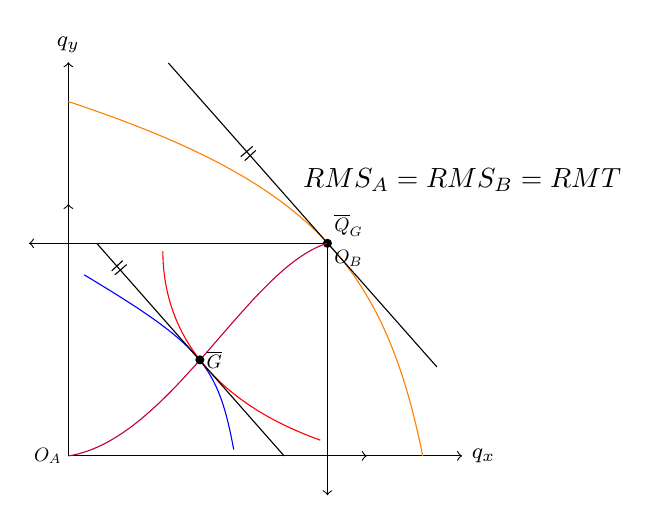
\begin{tikzpicture}
	% FPP
		% Ejes
			\draw[->] (10,0)-- (10,5) node[align=center, above] {\footnotesize $q_{y}$};
			\draw[->] (10,0) -- (15,0) node[align=center, right] {\footnotesize $q_{x}$};
		% Curva
			\draw [orange] (10,4.5) ..controls (13,3.5) and (14,2.5) .. (14.5,0);
			
	% Minicaja
		% Intersección
			\draw [<->] (9.5,2.7) -- (13.29,2.7) node [below right, scale=0.7] {$O_B$} -- (13.29,-0.5);
			\draw [<->] (10,3.2) -- (10,0) node [left, scale=0.7] {$O_A$} -- (13.79,0);
		% Puntos
			\draw[black, fill=black] (13.29,2.7) circle[radius=0.05] node [above right, scale=0.7] {$\overline{Q}_G$};
		% Curva de contrato
			\draw [purple] (10,0) ..controls (11.29,0.2) and (12.29,2.4) .. (13.29,2.7);
			\draw [blue] (10.2,2.3) ..  controls (11.7,1.4) and (11.9,1.15) .. (12.1,0.08);
			\draw [red] (11.2,2.6) ..  controls (11.2,1.6) and (11.8,0.7) .. (13.2,0.2);
		% Pendientes
			\draw (11.27,4.99) -- (14.68,1.13);
			\draw (10.36,2.7) -- (12.74,0);
		% Símbolo de paraleleas
			\draw (10.55,2.35) -- (10.69,2.48);
			\draw (10.59,2.3) -- (10.74,2.43);
			
			\draw (12.19,3.8) -- (12.34,3.93);
			\draw (12.24,3.75) -- (12.38,3.88);
		% 	Etqiueta
			\draw (15, 3.5) node {$RMS_A = RMS_B = RMT$};
		% Punto
			\draw[black, fill=black] (11.67,1.22) circle[radius=0.05] node [right, scale=0.7] {$\overline{G}$};
\end{tikzpicture}
\end{frame}
%------------------------------------------------
\begin{frame}{Asignación eficiente en sentido de Pareto}
	Es una asignación factible, tal que no existe otra asignación factible donde se pueda mejorar al menos a un consumidor sin empeorar a nadie. Por tanto, dada la utilidad de uno de los agentes, se tiene que estar maximizando la utilidad del otro, sujeto a las restricciones de factibilidad y a que la utilidad del primer agente es igual o superior a un determinado nivel.\\
	\bigskip
	Una asignación $(x_{1}^{A},x_{2}^{A}, x_{1}^{B},x_{2}^{B})$ es eficiente en sentido de Pareto si y solo si satisface OP.
	
		\begin{align*}
			& \text{Max } \quad u^{A}\left(x_{1}^{A},x_{2}^{A}\right) \\
			& \begin{array}{ll}
				\text{s.a: } & u^{B}\left(x_{1}^{B},x_{2}^{B} \right) = \overline{u}^{B}\\
				& x_{1}^{A}+x_{1}^{B} = \overline{w}_1  \\
				& x_{2}^{A}+x_{2}^{B} = \overline{w}_2  
			\end{array}
		\end{align*}
\end{frame}
%------------------------------------------------
\begin{frame}{Asignación eficiente en sentido de Pareto}
	El punto $D$ es una asignación de mayor utilidad pero no es eficiente. El punto $E$ es una asignación eficiente. $G$ también es una posible asignación eficiente \\
		\vspace{-0.6cm}
	\begin{tikzpicture}[scale=1.1]
	% Formación de la caja
		% Consumidor A
			\draw[->] (0.5,0.5) node[align=center, below left] {\footnotesize $O_J$} -- (0.5,4.5) node[align=center, above] {\footnotesize $6R$};
			\draw[->] (0.5,0.5) -- (8.5,0.5) node[align=center, right] {\footnotesize $10A$};
		
		% Consumidor B
			\draw[->] (8,4) node[align=center, above right] {\footnotesize $O_K$} -- (0,4) node[align=center, left] {\footnotesize $10A$};
			\draw[->] (8,4) -- (8,0) node[align=center, below] {\footnotesize $6R$};
			
		% Flechas
			\node[draw, single arrow,
				minimum height=22mm, minimum width=1mm,
				single arrow head extend=1.5mm,
				anchor=west, red, scale=0.5, rotate=-90,transform shape] at (8.4,2.87) {\small Ropa de Karen};
				
			\node[draw, single arrow,
				minimum height=22mm, minimum width=1mm,
				single arrow head extend=1.5mm,
				anchor=west, blue, scale=0.5, rotate=90,transform shape] at (0.1,1.57) {\small Ropa de Jaime};
				
			\node[draw, single arrow,
				minimum height=22mm, minimum width=1mm,
				single arrow head extend=1.5mm,
				anchor=west, red, scale=0.5, rotate=180,transform shape] at (5,4.3) {\rotatebox {180} {\small Alimento de Karen}};
			
			\node[draw, single arrow,
				minimum height=22mm, minimum width=1mm,
				single arrow head extend=1.5mm,
				anchor=west, blue, scale=0.5,transform shape] at (3.5,0.2) {\small Alimento de Jaime};
		
	% Curvas de indiferencia
		\begin{axis}[
					hide axis,
					xmin=0, xmax=10, 
					ymin=0, ymax=10,
					ytick=\empty,
					]
			
			% Área sombreada
				\fill [pattern=crosshatch dots,pattern color=green!60!white] (axis cs:4.07,6.462) to [bend right=34] coordinate[pos=0.5] (l_i) (axis cs:8.43,1.57) to (axis cs:8.42,1.56) to [bend right=34] coordinate[pos=0] (l_i) (axis cs:4,6.461);;
			
			% Curvas de indiferencia
				% Agente A
					\draw [blue] (axis cs:4,6.9) to [bend right=40] coordinate[pos=1] (l_i) (axis cs:9,1.5);
					\draw [blue] (axis cs:4.8,6.9) to [bend right=40] coordinate[pos=1] (l_i) (axis cs:9,2.3);
					\draw [blue] (axis cs:6.2,6.9) to [bend right=40] coordinate[pos=1] (l_i) (axis cs:9,3.7);
				
				% Agente B
					\draw [red] (axis cs:8.5,1) to [bend right=40] coordinate[pos=0.5] (l_i) (axis cs:3.6,6.5);
					\draw [red] (axis cs:8,1) to [bend right=40] coordinate[pos=0.5] (l_i) (axis cs:3.6,6);
					\draw [red] (axis cs:7.1,1) to [bend right=40] coordinate[pos=0.5] (l_i) (axis cs:3.6,5.1);
					\draw [red] (axis cs:6.3,1) to [bend right=40] coordinate[pos=0.5] (l_i) (axis cs:3.6,4.3);
		\end{axis}
	
	% Punto
		\draw[black, fill=black] (5.775,0.89) circle[radius=0.05] node [above right] {$C$};
		\draw[black, fill=black] (5.26,1.47) circle[radius=0.05] node [above right] {$D$};
		\draw[black, fill=black] (4.1,2.2) circle[radius=0.05] node [above right] {$E$};
		\draw[black, fill=black] (3.7,1.9) circle[radius=0.05] node [below left] {$F$};
		\draw[black, fill=black] (4.82,2.7) circle[radius=0.05] node [above right] {$G$};
	
	% Etiqueta de función de utilidad
		% Agente A
			\node [blue, scale=0.18mm]  at (6.35,0.8) {$u_{J}^{1}$};
			\node [blue, scale=0.18mm]  at (6.35,1.27) {$u_{J}^{1}$};
			\node [blue, scale=0.18mm]  at (6.35,2.06) {$u_{J}^{1}$};
			
		% Agente B
			\node [red, scale=0.18mm]  at (2.3,3.8) {$u_{K}^{1}$};
			\node [red, scale=0.18mm]  at (2.3,3.5) {$u_{K}^{2}$};
			\node [red, scale=0.18mm]  at (2.3,3) {$u_{K}^{3}$};
			\node [red, scale=0.18mm]  at (2.3,2.55) {$u_{K}^{4}$};
	
\end{tikzpicture}
\end{frame}
%------------------------------------------------
\begin{frame}{Eficiencia en el intercambio}
	\begin{itemize}
		\item Cualquier movimiento fuera de la lente sombreada empeorará a algún agente.
		\item B es un intercambio mutuamente beneficioso —ambos agentes alcanzan curvas de indiferencia de mayor utilidad que su dotación inicial— pero no es eficiente.
		\item Por tanto, el intercambio puede ser beneficioso pero no necesariamente eficiente.
		\item Las RMS son iguales cuando las curvas de indiferencia son tangentes y,por tanto, la asignación es eficiente.
	\end{itemize}
\end{frame}
%------------------------------------------------
\begin{frame}{La eficiencia paretiana significa que}
	\begin{itemize}
		\item No hay forma de hacer que todas las personas mejoren.
		\item No hay forma que una persona mejore sin que al menos otra persona empeore.
		\item Todas las ganancias del intercambio han sido agotadas.
	\end{itemize}
\end{frame}
